\section{Теорема об изменении механической энергии}

\begin{wrapfigure}{r}{4cm}
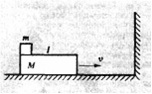
\includegraphics[width=4cm]{0601MechanicalEnergyBlocks.jpg}
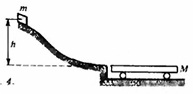
\includegraphics[width=4cm]{0602MechanicalEnergyHill.jpg}
\end{wrapfigure}

%1
\AddProb На бруске длиной $l$ массой $M$, расположенном на гладкой горизонтальной поверхности, лежит маленькое тело массой $m$. 
Коэффициент трения между телом и бруском $\mu$. С какой скоростью $v$ должна двигаться система, 
чтобы после упругого удара бруска о стенку тело упало с бруска?

\AddProb Тело массой $m$ съезжает с высоты $h$ гладкой наклонной плоскости и начинает скользить по тележке массой $M$, 
находяжейся на гладкой горизонтальной поверхности. Коэффициент трения между телом и тележкой $\mu$. 
На какое расстояние переместится тело относительно тележки?

\begin{wrapfigure}{r}{4cm}
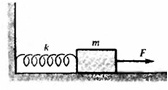
\includegraphics[width=4cm]{0603MechanicalEnergySpring.jpg}
\end{wrapfigure}

\AddProb На горизонтальной плоскости лежит тело массой $m$, соединенное с вертикальной стеной пружиной жесткостью $k$. 
В начальный момент времени пружина не деформирована. На тело начинает действовать постоянная сила $F$. 
Считая, что коэффициент трения между телом и плоскостью $\mu$ и что $F >\mu mg$, 
найдите максимальное смещение тела от начального положения и максимальную скорость тела в процессе движения.

\begin{wrapfigure}{r}{4cm}
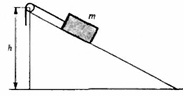
\includegraphics[width=4cm]{0604MechanicalEnergyWedgeAndBlock.jpg}
\end{wrapfigure}

\AddProb Груз массой $m$ медленно поднимают на высоту $h$ по наклоной плоскости с помощью блока и троса. 
При этом совершается работа $A$. Затем трос отпускают, и груз скользит вниз. Найдите величину $A$, если известно, 
что скорость тела в конце спуска равна $v$.

\AddProb (2010) У основания наклонной плоскости находится брусок. Бруску сообщают некоторую начальную скорость, 
направленную вдоль плоскости вверх. На высоте $h$ скорость бруска уменьшается до значения $v_1$. 
После абсолютно упругого удара о стенку, расположенную на высоте $H > h$, брусок скользит вниз, 
и на той же высоте $h$ его скорость равна $v_2<v_1$. Определите скорость бруска в момент удара о стенку.


\section{Энергия и импульс}
%6
\AddProb На гладкой горизонтальной поверхности лежит небольшая шайба массы $m$ и гладкая горка массы $M$ высоты $H$. 
Какую минимальную скорость $v$ надо придать шайбе, чтобы она смогла преодолеть барьер?

\AddProb (2012) Две лодки идут параллельными курсами навстречу друг другу с одинаковыми скоростями $v$. 
Когда лодки встречаются, с одной лодки на другую перебрасывают груз массой $m$, а затем со второй лодки на первую перебрасывают такой же груз. 
В другой раз грузы перебрасывают из лодки в лодку одновременно. В каком случае скорости лодок после перебрасывания грузов будут больше? 
Масса каждой лодки $M$.

\AddProb (2006) Лягушка массы $m$ сидит на конце доски массы $M$ и длины $L$. Доска плавает по поверхности пруда. 
Лягушка прыгает под углом $\alpha$ к горизонту вдоль доски. Какой должна быть начальная скорость лягушки, 
чтобы она оказалась после прыжка на противоположном конце доски? Как изменится ответ, если 1) доска и лягушка сносятся течением со скоростью $u$,
 и лягушка прыгает по направлению против течения; 2) доска испытывает при своем движении постоянную силу сопротивления воды $F$?

\AddProb (2001) Трактор массы $m$ рывками перемещает груз массы $M>m$. Они соединены прочным нерастяжимым тросом длины $L$. 
В начальный момент трактор находится рядом с грузом. Сколько рывков надо сделать трактору, чтобы переместить его на расстояние $s$? 
Считать, что коэффициент трения трактора и груза о землю одинаков.

\AddProb Два груза массы $m$, соединенные пружиной жесткостью $k$, находятся на гладком горизонтальном столе. 
Одному из тел сообщают скорость $v$ и измеряют максимальное растяжение пружины. 
В ходе опыта пружина лопнула при растяжении, равном половине максимального. С какими скоростями грузы поедут по столу?

\begin{wrapfigure}{r}{4cm}
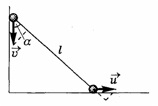
\includegraphics[width=4cm]{0611EnergyAndImpulseBar.jpg}
\end{wrapfigure}

%11
\AddProb Два тела малых размеров массой $m$ каждое соединены стержнем пренебрежимо малой массы длиной $l$. 
Система из начального положения у вертикальной гладкой стены приходит в движение. 
Нижнее тело скользит без трения по горизонтальной поверхности, верхнее - по вертикальной. 
Найдите значение скорости нижнего тела, при котором верхнее оторвется от вертикальной стенки.

\begin{wrapfigure}{r}{2.5cm}
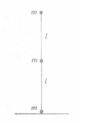
\includegraphics{0612EnergyAndImpulseBalls.jpg}
\end{wrapfigure}

\AddProb (2002) Три одинаковых шарика массы $m$ каждый, скрепленные двумя невесомыми стержнями длиной $l$, 
поставили на гладкую горизонтальную плоскость. Найти скорость верхнего шарика в момент удара о плоскость.